% Referencias - con imagen de fondo específica
\cleardoublepage\thispagestyle{empty}
\refstepcounter{chapter}
\phantomsection\addcontentsline{toc}{chapter}{Referencias}\label{cap:referencias}

% Imagen de fondo específica para referencias
\AddToShipoutPicture*{%
	\put(0,0){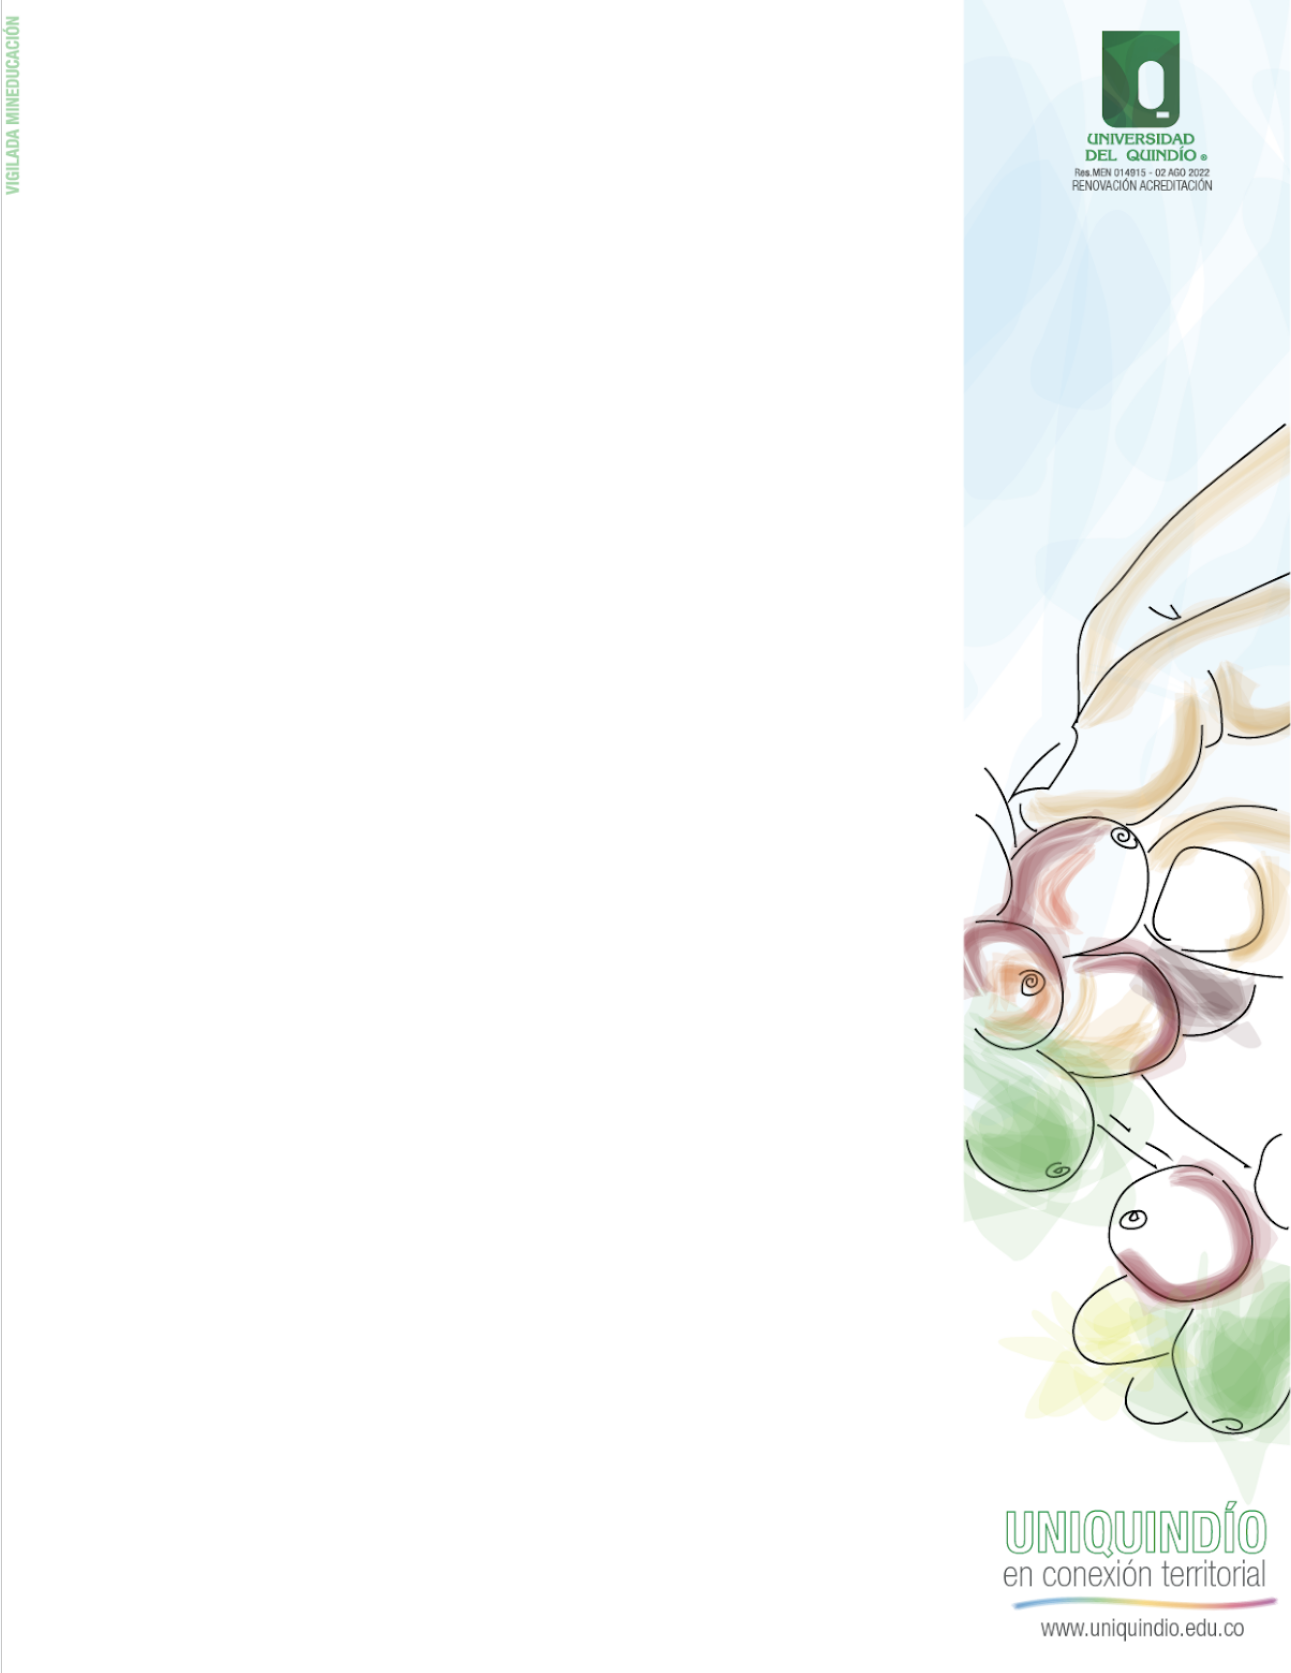
\includegraphics[width=\paperwidth,height=\paperheight]{./images/referencias.png}}%
}

% Título posicionado con coordenadas absolutas (en píxeles desde esquina superior izquierda)
\begin{tikzpicture}[remember picture,overlay]
	\node[anchor=north west] at ([xshift=150pt,yshift=-370pt]current page.north west)
	{\Large\bfseries\textcolor{black}{Referencias}};
\end{tikzpicture}
\vspace{2cm}

% Bibliografía sin título automático
\begingroup
\renewcommand{\bibname}{}
\pagestyle{fancy} % Fuerza el estilo fancy para todas las páginas de bibliografía
\bibliographystyle{apalike-impure-es}
\bibliography{bibliografia}
\endgroup

\newpage
